\documentclass{beamer}
\usepackage[russian]{babel}
\usetheme{metropolis}

\usepackage{amsthm}
\setbeamertemplate{theorems}[numbered]

\setbeamercolor{block title}{use=structure,fg=white,bg=gray!75!black}
\setbeamercolor{block body}{use=structure,fg=black,bg=gray!20!white}

\usepackage[T2A]{fontenc}
\usepackage[utf8]{inputenc}

\usepackage{hyphenat}
\usepackage{amsmath}
\usepackage{graphicx}

\AtBeginEnvironment{proof}{\renewcommand{\qedsymbol}{}}{}{}

\title{
Микроэкономика-I
}
\author{
Павел Андреянов, PhD
}

\begin{document}

\maketitle

\section{Технологические множества}

\begin{frame}{Технологические множества}

В первой части мы фокусировались на минимизации издержек, однако это накладывало определенные ограничения, поскольку описать технологию просто можно одним из двух способов:
$$ x = G(\vec y), \quad F(\vec x) = y,$$
то есть либо один фактор, либо один конечный товар. Нам хотелось бы описать более сложные технологии, в которых есть много факторов и много конечных товаров.

\end{frame}

\begin{frame}{Технологические множества}

Оказывается, что удобнее всего отказаться от разделения между факторами и товарами и думать о них одинаково, а наша технология будет описывать, как можно одни товары превращать в другие.

Пусть есть $n$ товаров, которые можно произвести в количествах, описываемых точкой в $\mathbb{R}^n$ (не в $\mathbb{R}^n_+$), поскольку какие-то товары окажутся факторами, потраченными при производстве других. 

\end{frame}

\begin{frame}{Технологические множества}

Одна технология – это одна точка. Множество всех допустимых технологий – это область в $\mathbb{R}^n$, то есть **технологическое множество**. Эффективное производство (то, что раньше описывалось $F$ или $G$) теперь описывается границей этого множества, то есть **технологической границей**, см. иллюстрацию ниже.

\end{frame}

\begin{frame}{Технологические множества}

\begin{figure}[hbt]
\centering
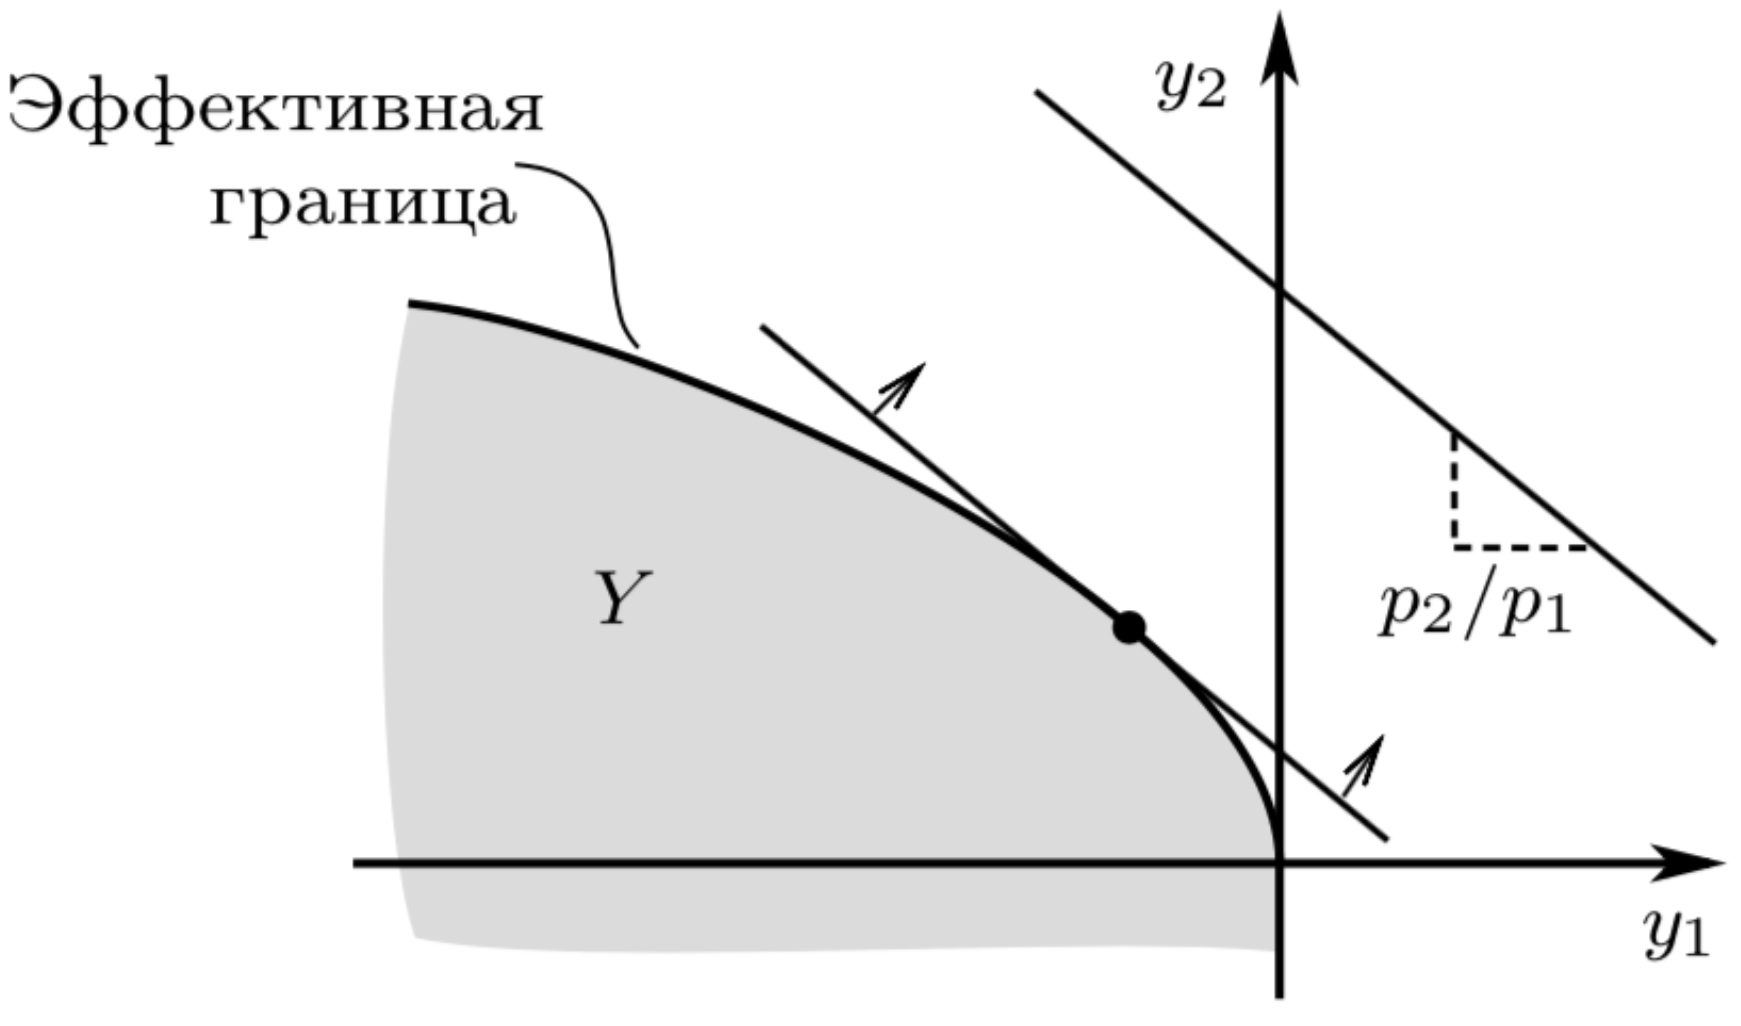
\includegraphics[width=.8 \textwidth]{prod_set.png}
\end{figure}

\end{frame}

\begin{frame}{Технологические множества}

Формально технологическая граница состоит из точек $y \in Y$, таких, что не существует $y' \in Y$, так что $y_i' \geqslant y_i$ по всем координатам $i$ и $y_j' > y_j$ по хотя бы одной координате $j$.

\begin{lemma}
Технологическая граница ищется как все точки $z \in Y$ т.ч.
$$ z \in \text{argmax } \vec q \cdot \vec y, \quad \vec y \in Y,$$
для хотя бы одного вектора цен $\vec q \geqslant 0, \vec q \neq 0$.
\end{lemma}
\end{frame}

\section{Аксиомы производителя}

\begin{frame}{Аксиомы производителя}

Фирма воспринимает технологическое множество и максимизирует прибыль:
$$ \vec q \cdot y \to \max, \quad \vec y \in Y.$$
Чтобы задача была выпуклой, нам понадобятся некоторые аксиомы.

\end{frame}

\begin{frame}{Аксиомы производителя}

\begin{definition}
Аксиомы технологического множества $Y$:

- A1: $Y$ содержит $\vec{0}$
- A2: свобода расходования
$$ y \in Y, y' < y \quad \Rightarrow \quad y' \in Y$$

- A3: невозрастающая отдача от масштаба:
$$y \in Y \Rightarrow \lambda Y \in Y, \quad \forall \lambda \in (0,1)$$

- A4: непусто, замкнуто

- A5: отсутствие рога изобилия: $Y \cap \mathbb{R}^n_{+} = \emptyset$.
\end{definition}

\end{frame}

\begin{frame}{Аксиомы производителя}

Все эти аксиомы нужны, чтобы вывести из них свойства задачи максимизации полезности, которые нам хорошо известны наперед: непрерывность и выпуклость. Гладкость тоже желательна, но, на самом деле, можно обойтись выпуклостью $Y$, поскольку выпуклые функции почти всюду дифференцируемы.

\end{frame}

\begin{frame}{Аксиомы производителя}
\begin{theorem}[БЖЦ]

Если выполнены аксиомы A1-A5, то технологическое множество выпукло. Более того, если производится один товар, то функция $F$, описывающая технологическую границу, непрерывна и вогнута.
\end{theorem}

\end{frame}

\section{Максимизация полезности}

\begin{frame}{Максимизация полезности}
В такой абстрактной постановке удобно анализировать задачу максимизации полезности:
$$ \pi(q, y) = \vec q \cdot \vec y \to \max, \quad y \in Y$$

Как обычно, нас интересуют два объекта:

\begin{itemize}
\item координаты оптимума $y^{\ast}(\vec q)$ - это \textbf{функция предложения}
\item значение целевой функции $\pi^{\ast}(\vec q) = \pi(\vec q, y^{\ast}(\vec q)))$
\end{itemize}

\end{frame}

\begin{frame}{Максимизация полезности}

В такой абстрактной постановке удобно анализировать задачу максимизации полезности:

$$ \pi(q, y) = \vec q \cdot \vec y \to \max, \quad y \in Y$$

Как обычно, нас интересуют два объекта:

\begin{itemize}
\item координаты оптимума $y^{\ast}(\vec q)$ - это \textbf{функция предложения}
\item значение целевой функции $\pi^{\ast}(\vec q) = \pi(\vec q, y^{\ast}(\vec q)))$
\end{itemize}

Поскольку тут происходит огибание в пространстве $\vec q$, постарайтесь ответить на следующие два вопроса:

Вопрос: Чему равен градиент $\pi^{\ast}(\vec q)$?

Вопрос: Какова форма функции $\pi^{\ast}(\vec q)$?

\end{frame}

\section{Максимизация полезности}

\section{Сложение технологических множеств}

\begin{frame}{Сложение технологических множеств}

Предположим, что у нас есть два завода. Первый обладает технологией $Y_1$, второй обладает технологией $Y_2$. Теперь представим себе, что компания владеет этими двумя заводами и может свободно перемещать товары с одного завода на другой и комбинировать любые технологические цепочки. 

Как описать технологическое множество $Y_1 + Y_2$, соответствующее этой компании?

\end{frame}

\begin{frame}{Сложение технологических множеств}

\begin{definition}
Для двух множества $A$ и $B$, их \textbf{евклидова сумма} $A+B$ определяется как:
$$ A+B = \{a + b \ | \ a \in A, \ b \in b\}.$$
\end{definition}
\end{frame}

\begin{frame}{Сложение технологических множеств}
Действительно, компания может <<сложить>> в векторном смысле любые два вектора из множеств $A, B$. 

Первый вектор $a \in A$ означает, что партия товаров была произведена на первом заводе и была отправлена на склад. Второй вектор $b \in B$ означает, что партия товаров была произведена на втором заводе и тоже отправлена на склад. 

На складе партии будут объединены и суммарный объем будет соответствовать вектору $a + b$.
\end{frame}

\begin{frame}{Сложение технологических множеств}
\begin{lemma}
Арифметическая сумма двух выпуклых множеств выпукла.
\end{lemma}
Любая взвешенная сумма двух векторов из $A+B$ представляется как сумма двух взвешенных пар векторов из $A$ и $B$ с теми же весами.
$$ \alpha(a + b) + (1-\alpha)(a'+b') = [\alpha a + (1-\alpha) a'] + [\alpha b + (1-\alpha) b']$$
Соответственно, она тоже лежит в $A + B$.
\end{frame}

\section{Сложение технологических границ}

\begin{frame}{Сложение технологических границ}

Предположим далее, что $Y_1$ описывается производственной функцией $F_1$, а $Y_2$ описывается производственной функцией $F_2$. Как будет выглядеть производственная функция для $Y_1 + Y_2$?

Какие есть кандидаты?

- $F_1 + F_2$
- $\max(F_1 + F_2)$
- $\nabla F_1 = \nabla F_2$

\end{frame}

\begin{frame}{Сложение технологических границ}

Легко видеть, что производственная функция $F$ множества $Y_1 + Y_2$ определяется как верхняя огибающая семейства опорных функций: $$F(x_1, \ldots, x_n) : = \max_{\hat x} \left(F_1(\hat x_1, \ldots, \hat x_n) + F_2(x_1 - \hat x_1, \ldots, x_n - \hat x_n)\right),$$

то есть мы сначала решаем сколько произвести на первом заводе, а потом производим остальное на втором заводе. Что нам говорит Теорема об Огибающей?

\end{frame}

\begin{frame}{Сложение технологических границ}

Наклон огибающей равен наклону опорной функции в точке касания:
$$ \nabla F = \nabla F_2.$$

\end{frame}

\begin{frame}{Сложение технологических границ}

С другой стороны, можно сказать, что
$$F(x_1, \ldots, x_n) : = \max_{\hat x} \left(F_2(\hat x_1, \ldots, \hat x_n) + F_1(x_1 - \hat x_1, \ldots, x_n - \hat x_n)\right),$$

то есть мы сначала решаем сколько произвести на первом заводе, а потом производим остальное на втором заводе

\end{frame}

\begin{frame}{Сложение технологических границ}
И снова Теорема об Огибающей:
$$ \nabla F = \nabla F_1.$$

\end{frame}

\begin{frame}{Сложение технологических границ}
Получается, что необходимым условием для того, чтобы точка лежала на границе объединенного технологического множества $\vec y \in Y_1 + Y_2$ является то, что, при разложении $\vec y = \vec y_1 + \vec y_2$ этой точки на вектор $\vec y_1 \in Y_1$ и вектор $\vec y_2 \in Y_2$:
$$ \nabla F_1(\vec y_1) =  \nabla F_2(\vec y_2).$$

\end{frame}

\begin{frame}{Сложение технологических границ}
С другой стороны, очевидно, что при разложении $\vec y = \vec y_1 + \vec y_2$ этой точки, $\vec y_1$ на границе $Y_1$, а $\vec y_2$ лежит на границе $Y_2$. 

Таким образом, для того, чтобы описать суммарную технологическую границу, надо сложить только те пары точек $y_1 = F_1(\vec x_1)$ и $y_2 \in F_2(\vec x_2)$, в которых наклоны равны, и сосчитать $(\vec x_1 + \vec x_2, y_1 + y_2)$.

\end{frame}

\section{Конец}

\end{document}